\begin{quote}
Things in motion sooner catch the eye\\
Than what not stirs. --W.S., ``Troilus and Cressida'' 
\end{quote}

Old objects will sometime reveal new secrets when put in motion. In 2011 we uploaded a video \cite{dsr_vid11d} showing the family of 3-periodic {\em orbits} in an Elliptic Billiard  \cite{sergei91,birkhoff66}. We drew the locus of the {\em Incenter} and intouch points \cite{mw}. The former describes an ellipse while the latter is more complex, with two internal self-intersecting lobes, Figure~\ref{fig:intro-plot}.

\begin{figure}
    \centering
    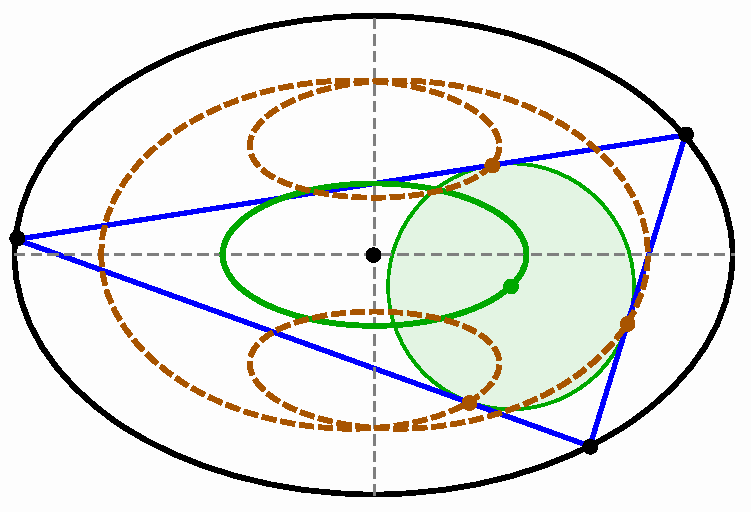
\includegraphics[width=.5\textwidth]{pics/0001_intro_plot.pdf}
    \caption{An $N=3$ orbit (blue), its Incircle (transparent green), Incenter (green dot) and contact points (brown dots) are shown. Over the $N=3$ family, the Incenter locus is an ellipse (green), and that of the intouch points is a self-intersecting curve with two internal lobes (dashed brown).}
    \label{fig:intro-plot}
\end{figure}

Over the next few years there surfaced elegant proofs for the ellipticity of the Incenter \cite{olga14,ronaldo16} as well as for that of the Barycenter \cite{sergei2016,ronaldo19}, Circumcenter  \cite{corentin19,ronaldo19}, and Orthocenter \cite{ronaldo19}.

Here we describe a second exploratory cycle, some eight years after our original video. As before, we began with loci of Triangular Centers \cite{mw}. The curves we obtained went from expected, to new, to amazing: elliptic, non-elliptic, quasi-elliptic, with kinks, similar or identical to the Billiard (or its Caustic), point-like, and even perfectly circular!

Beyond loci, $N=3$ revealed an amazing property: the ratio of Inradius to Circumradius is invariant, and this implies beautiful relations involving orbit angles and areas.
Here,  invariant means that the property is shared for all 3-periodic orbits of the billiard. Other suprising invariants were that the $N=3$ family has a stationary Mittenpunkt \cite{mw} and a stationary Cosine Circle \cite{mw}. 

Close observation of the $N=4$ family, closely related to Monge's Orthoptic Circle \cite{connes07}, Figure~\ref{fig:monge-orthoptic}, provided us clues with which to generalize all $N=3$ thus found for all $N$, namely the fact that these two (i) contain a stationary point, (ii) a stationary circle, and (iii) preserve angular and area relations. These investigations are summarized in Figure~\ref{fig:global-diagram}.

\begin{figure}[H]
    \centering
    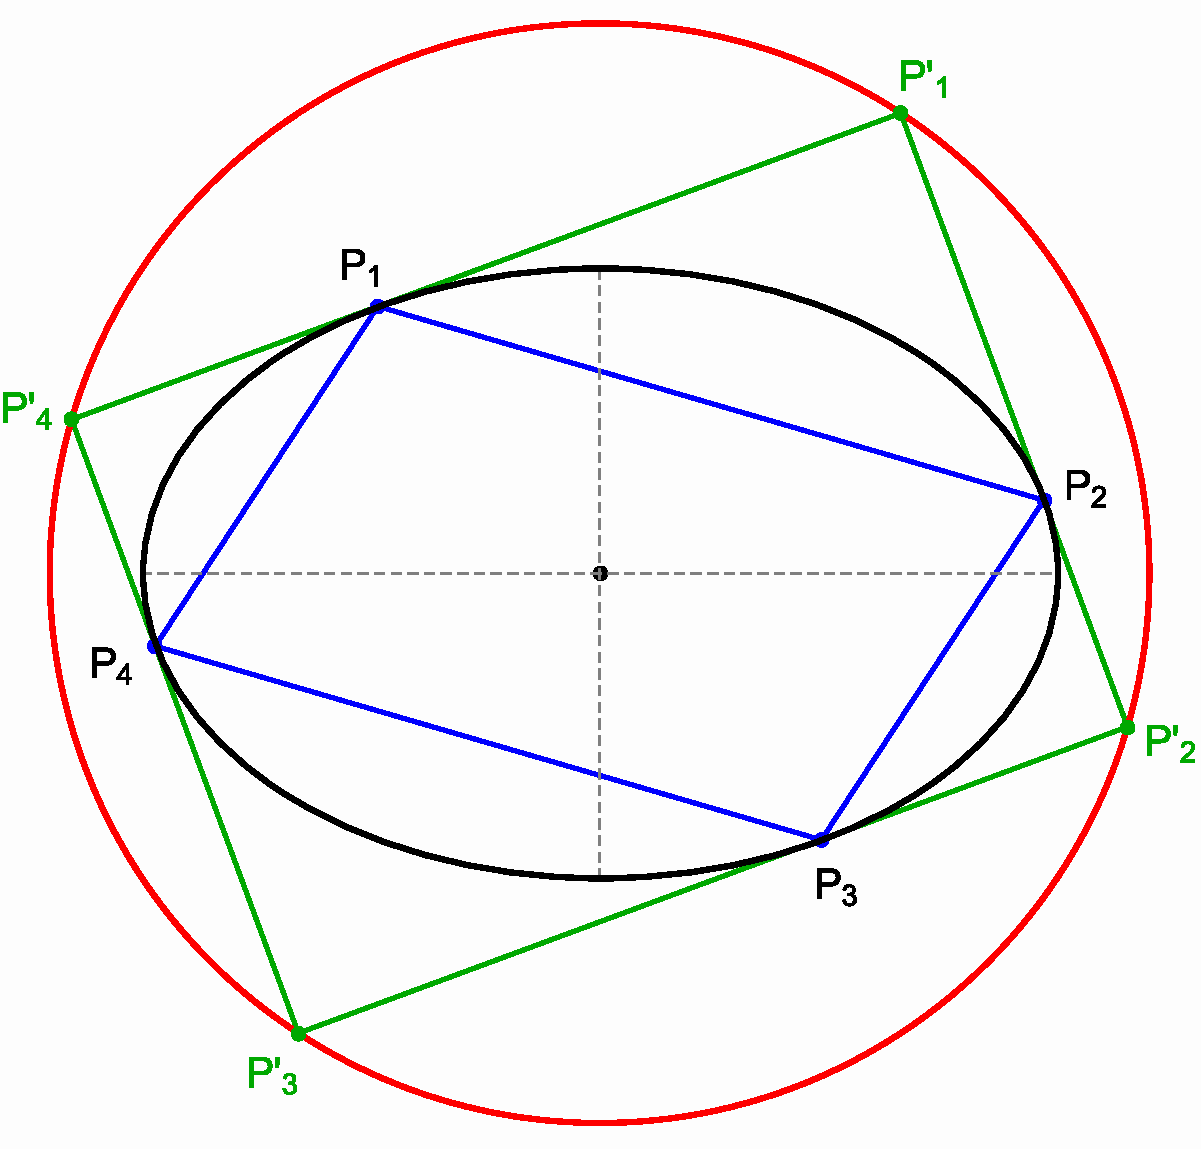
\includegraphics[width=.4\textwidth]{pics/0200_monge_orthoptic.pdf}
    \caption{French Mathematician Gaspard Monge (1746-1818) discovered that the locus of points whose tangents to a given ellipse subtend a right angle is a circle (red). Here's the connection to Billiards: take a point $P_1'$ on Monge's Circle and extend one tangent till it hits the circle again $P_2'$. Repeat this twice so as to yield four vertices on the circle. Suprisingly, these form a rectangle, and its four points of tangency $P_1P_2P_3P_4$ define an inscribed parallelogram  which is a billiard orbit of the ellipse! Note: the family of $N=4$ billiard orbits are constant-perimeter parallelograms.}
    \label{fig:monge-orthoptic}
\end{figure}

\begin{figure}[H]
    \centering
    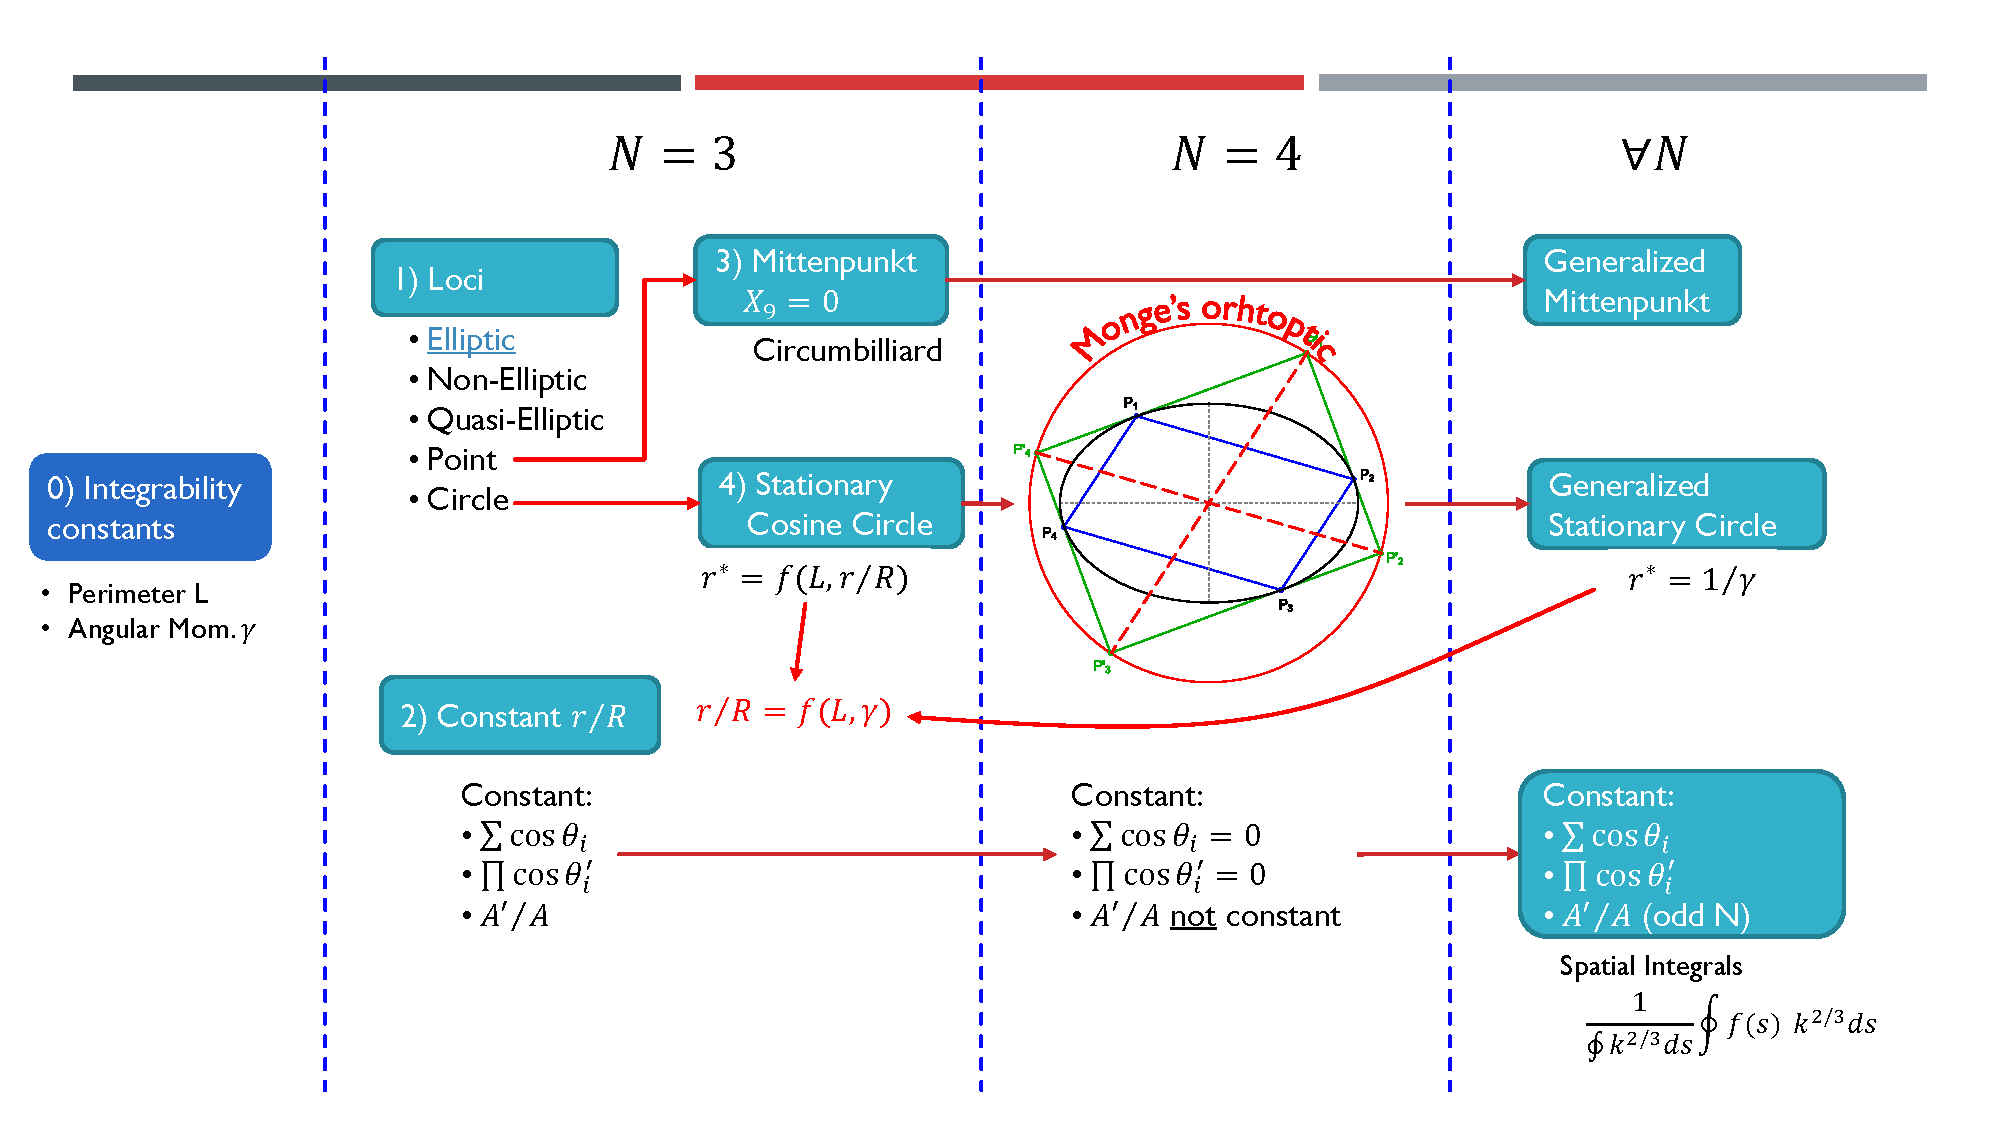
\includegraphics[width=\textwidth]{pics/0002_diagram_slide.pdf}
    \caption{A bird's eye view of our exploration. From left to right: (i) we start with know results from the integrability of the Elliptic Billiard, namely constant orbit perimeter $L$ and constant Joachmisthal's angular momentum $\gamma$. We then (ii) investigate various properties of the $N=3$ family. (iii) Close observation of the $N=4$ family provides clues to (iv) generalizations of all propertiees $\forall{N}$. A key unification (red arrows) is expressing $r/R$ in terms of $S$ and $\gamma$.}
    \label{fig:global-diagram}
\end{figure}

In the remainder of this paper we will describe our explorations in the following order:

\begin{itemize}
    \item Beautiful elliptic and non-elliptic loci.
    \item The Mittenpunkt: a point-like locus.
    \item The $r/R$ invariant and its corollaries.
    \item The Cosine Circle: a circular locus.
    \item Generalizing all results to $N>3$.
\end{itemize}

Many of our key observations are available as online videos, images, and applets \cite{reznik_media}. We also maintain a companion website \cite{reznik_web} where details about this work are constantly added and/or updated.